%-----------------------------------LICENSE------------------------------------%
%   This file is part of tikz_figures.                                         %
%                                                                              %
%   tikz_figures is free software: you can redistribute it and/or              %
%   modify it it under the terms of the GNU General Public License as          %
%   published by the Free Software Foundation, either version 3 of the         %
%   License, or (at your option) any later version.                            %
%                                                                              %
%   tikz_figures is distributed in the hope that it will be useful,            %
%   but WITHOUT ANY WARRANTY; without even the implied warranty of             %
%   MERCHANTABILITY or FITNESS FOR A PARTICULAR PURPOSE.  See the              %
%   GNU General Public License for more details.                               %
%                                                                              %
%   You should have received a copy of the GNU General Public License along    %
%   with tikz_figures.  If not, see <https://www.gnu.org/licenses/>.           %
%------------------------------------------------------------------------------%

% Use the standalone class for displaying the tikz image on a small PDF.
\documentclass[crop, tikz]{standalone}

% Import the tikz package to use for the drawing.
\usepackage{tikz}

% Tikz packages used.
\usetikzlibrary{arrows.meta}

% Begin the document.
\begin{document}

    % Draw the figure.
    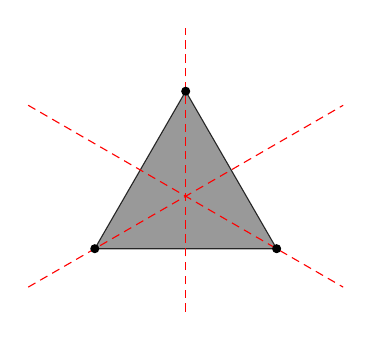
\begin{tikzpicture}[> = Latex]

        % Defining points for the triangle.
        \coordinate (A) at (0.0, 1.0);
        \coordinate (B) at (1.1547, -1.0);
        \coordinate (C) at (-1.1547, -1.0);

        % Fill in the triangle.
        \draw[fill = gray, opacity = 0.8] (A) to (B) to (C) to cycle;

        % Mark the lines of reflection.
        \draw[densely dashed, draw = red] (-2.0, -1.4880) to (2.0,  0.8213);
        \draw[densely dashed, draw = red] (-2.0,  0.8213) to (2.0, -1.4880);
        \draw[densely dashed, draw = red] (0.0, -1.8000) to (0.0,  1.8000);

        % Place dots at the vertices.
        \draw[fill = black] (A) circle (0.05);
        \draw[fill = black] (B) circle (0.05);
        \draw[fill = black] (C) circle (0.05);
    \end{tikzpicture}
\end{document}
